\documentclass[11pt]{article}

% ===== MSOM-compliant formatting =====
% 11pt, one-inch margins, double spacing (<=33 lines/page), single column,
% author-year citations, no footnotes. 32-page cap incl. references, tables,
% and appendices; heavy derivations live in the separate e-companion
% (ecompanion.tex, <=16 pages).
\usepackage[margin=1in]{geometry}
\usepackage{setspace}
\doublespacing

\emergencystretch 3em

% Images and plots
\usepackage{graphicx}
% Prefer vector art: figures are included without an extension so LaTeX picks
% the PDF when one exists and falls back to the raster preview otherwise.
% INFORMS requires vector PDF/EPS for plots (style instructions Sec. 9.1);
% only genuine images (the hand-drawn logistics diagram) stay raster.
\DeclareGraphicsExtensions{.pdf,.png,.jpg,.jpeg}
\usepackage{float}
\usepackage{subcaption}

% Float placement: let figures pack near their references rather than
% piling up one-per-page in the double-spaced layout.
\renewcommand{\topfraction}{0.9}
\renewcommand{\bottomfraction}{0.9}
\renewcommand{\textfraction}{0.08}
\renewcommand{\floatpagefraction}{0.75}
\setcounter{topnumber}{3}
\setcounter{bottomnumber}{2}
\setcounter{totalnumber}{5}

% Math
\usepackage{amsmath,amssymb,amsthm,enumitem,mathtools}
\renewcommand{\qedsymbol}{$\blacksquare$}

% Tables
\usepackage{booktabs}
\usepackage{multirow}

% Author-year citations (MSOM requirement)
\usepackage[round,authoryear]{natbib}
\bibliographystyle{plainnat}

% Hyperreferences
\usepackage[colorlinks=true, citecolor=blue, linkcolor=blue, urlcolor=blue]{hyperref}

% Acronyms / glossaries (group standard)
\usepackage[acronyms]{glossaries}
\makeglossaries

% Draft notes (hidden by commenting the second definition)
\newcommand{\mynote}[1]{\textcolor{blue}{\textbf{[note: #1]}}}
\usepackage{xcolor}

% Definitions (group math macros + theorem environments + acronyms)
\input{definitions.tex}

% Cross-references into the e-companion
\newcommand{\EC}{EC}

\title{\textbf{Robust Antimicrobial Supply Chain Design under\\ Epidemiological Demand Uncertainty in Botswana}}

% For MSOM double-blind submission, comment out the author block below and
% submit anonymized. The names are retained here for the working / preprint
% version.
\author{%
Elliot S. Lee$^{1,2}$ \and
Stefan Clarke$^{2}$ \and
Khumo Seipone$^{3}$ \and
Lesego Busang$^{3}$ \and
Tiro Molefe$^{3}$ \and
Stanley Mapiki$^{3}$ \and
Kabelo Kgongwana$^{3}$ \and
Bene D. Anand Paramadhas$^{4}$ \and
Idah Seepo$^{4}$ \and
Bartolomeo Stellato$^{2}$
}
\date{%
\small
$^{1}$Haas School of Business, University of California, Berkeley \quad
$^{2}$Department of Operations Research and Financial Engineering, Princeton University\\
$^{3}$African Comprehensive HIV/AIDS Partnerships (ACHAP) \quad
$^{4}$Central Medical Stores, Ministry of Health, Botswana\\[1ex]
\today
}

\begin{document}
\maketitle

% ===================== STRUCTURED ABSTRACT (<= 300 words) =====================
\begin{abstract}
\noindent
\textit{Problem definition.}
National medical-stores agencies in low- and middle-income countries must allocate essential antimicrobials across a multi-echelon distribution network under demand that is uncertain, overdispersed, non-stationary, and shaped by infectious-disease dynamics.
We study how a central agency should route and pre-position antimicrobials to minimize unmet demand and cost when demand is both statistically uncertain and endogenously coupled to the epidemic its distribution is meant to control.
\noindent
\textit{Methodology/results.}
We formulate a multi-echelon, multi-period allocation model with static and adjustable robust versions, the latter using affine decision rules (ARO-ADR).
The core methodological step is a dualization yielding a tractable single-level mixed-integer program that, with a district decomposition that gives every district a dedicated allocation, scales to 614 facilities across 18 districts.
Demand comes from a Medical Demand Estimator calibrated to catchment populations and point-prevalence-survey data.
On simulations driven by real Central Medical Stores procurement records, the adaptive policy reduces average unmet demand by 84--86\% relative to a deterministic baseline and 52--54\% relative to static robust optimization, at a procurement premium of 0.9\% under illustrative unit costs and 6.4--6.5\% under actual prices.
A two-strain SEIR extension, in which treatment intensity depends on realized supply, preserves the policy ordering under epidemic-driven demand.
\noindent
\textit{Managerial implications.}
Adaptive recourse lifts service in every district, including the worst-served, for a modest procurement premium, and the value of adaptivity concentrates in an identifiable regime (high demand variability, moderate uncertainty budget), giving agencies a concrete calibration rule.
Because clinical stockout costs dwarf unit procurement, realized service is pinned by physical capacity rather than the shortage penalty, so the recommended policy is insensitive to the exact penalty.
The framework is a deployable decision-support tool whose benefits are best read as coverage gains.
\end{abstract}

\bigskip

\noindent\textbf{Key words:} robust optimization; adjustable robust optimization; healthcare operations; pharmaceutical supply chains; antimicrobial resistance; global health

\clearpage

% ============================ INTRODUCTION ============================
\section{Introduction}
\label{sec:intro}

We consider the problem faced by a national medical-stores agency that must distribute essential antimicrobials to a country's public health facilities under uncertain demand.
The agency procures drugs centrally and ships them, over a multi-echelon network of warehouses, hospitals, clinics, and health posts, to the point of care.
Its objective is to keep antimicrobials available where and when patients need them, at acceptable cost, despite demand that it cannot observe in advance.
This is the operating reality of the Central Medical Stores (CMS) in Botswana, whose distribution failures in 2025 culminated in a declared national public health emergency \citep{reut25}, and it is representative of pharmaceutical logistics across much of sub-Saharan Africa \citep{adebisi2022,olutuase2022}.

Three features make this allocation problem hard, and they are the features our model is built around.
First, antimicrobial demand is \emph{statistically difficult}: facility-level counts are overdispersed and non-stationary, and the agency rarely has the distributional information that stochastic-programming approaches assume.
Second, the network is \emph{large and heterogeneous}: a cost-minimizing objective treats a unit of unmet demand as equally costly wherever it falls, so nothing in the objective itself prevents shortfalls from settling on the districts that are most expensive to reach, and both tractability and the distribution of service must be designed in rather than assumed.
Third, demand is ultimately \emph{shaped by disease dynamics}: because antimicrobials treat infections, a stockout does not merely register as unmet demand in one period but can prolong infectiousness and alter future need, so a realistic evaluation of an allocation policy should subject it to epidemic-driven, non-stationary demand.

\paragraph{Approach.}
We formulate the agency's problem as a multi-echelon, multi-period network optimization and address demand uncertainty through robust optimization, which is the core of the paper.
Rather than committing shipments entirely in advance, we allow them to adapt to demand as it is revealed, using affine decision rules; we refer to the resulting policy as adjustable robust optimization with affine decision rules (ARO-ADR).
The central technical step is a dualization that converts the semi-infinite robust constraints into a finite system, yielding a single-level mixed-integer program that, together with a district decomposition that gives every district a dedicated allocation, remains solvable at national scale.
We drive the model with a Medical Demand Estimator (MDE) calibrated to catchment populations and point-prevalence-survey data.
Finally, to test the policies against demand that is not merely uncertain but epidemiologically driven, we couple the model to a two-strain susceptible-exposed-infectious-recovered (SEIR) system in which treatment intensity, and therefore future demand, depends on realized drug availability; we treat this coupling as an extension that stress-tests the framework rather than as its centerpiece.

\paragraph{Contributions.}
This paper makes three contributions.
\begin{enumerate}
\item \emph{A tractable robust multi-echelon allocation model at national scale.} We formulate the agency's problem and develop static and affinely-adjustable robust versions, then derive a single-level dual reformulation that, paired with a district decomposition that gives every district a dedicated allocation, gives a mixed-integer program solvable across 614 facilities and 18 districts within practical time limits. This is the technical core of the paper.
\item \emph{Empirical evaluation on real procurement data with actionable managerial guidance.} Driving the model with a demand estimator calibrated to survey data and with actual CMS consumption and pricing records, we show that adaptive recourse yields large coverage gains in every district, including the worst-served, at a modest procurement premium, and we characterize the regime in which adaptivity is worth its cost and the sense in which the recommended policy is insensitive to the shortage penalty.
\item \emph{An epidemic-driven-demand extension.} We couple the allocation model to a two-strain SEIR system in closed loop: each period's realized deliveries set the treatment rates that generate the next period's demand, so a policy faces the demand its own shortfalls create. We use it to test whether the policy ordering persists once demand responds to supply. We present this as a proof-of-concept extension rather than a validated epidemiological model, and read its results as coverage gains rather than changes to long-run resistance.
\end{enumerate}

\paragraph{Managerial takeaways.}
Three findings are directly actionable for a medical-stores agency.
The adaptive policy cuts average unmet demand by roughly three-quarters relative to current-practice deterministic planning, and it does so in \emph{every} district, including the worst-served, rather than trading rural for urban coverage.
The value of adaptivity is largest in a specific and identifiable regime, high demand variability and a moderate uncertainty budget, which tells an agency when the added modeling effort pays off and when a simpler static policy suffices.
Finally, because the clinical cost of an antimicrobial stockout far exceeds unit procurement cost, the operationally relevant regime is one in which realized service is limited by physical network capacity rather than by the shortage penalty, so the recommended policy is insensitive to the precise penalty an agency assigns.

\paragraph{Related literature.}
Our work sits at the intersection of three streams.
The first is robust and adjustable robust optimization for inventory and supply chains: budgeted uncertainty sets \citep{bertsim04}, their tractable robust counterparts \citep{bental}, and affine decision rules for multistage adaptivity \citep{yanikoglu2018aro}.
We use this machinery but apply it to a network with endogenous, epidemiologically-driven demand, which is where our modeling novelty lies rather than in the robust apparatus itself.
The second is healthcare and humanitarian operations under epidemic uncertainty, including prescriptive analytics for pandemic response \citep{bertsimas21} and resource allocation under outbreak-driven demand \citep{govindan20}, together with the pharmaceutical-supply-chain reliability and resilience literature \citep{tkr22,ivanov22}.
The third is the modeling of antimicrobial resistance as a dynamic externality of treatment \citep{lax01,kd20}, and the statistics of overdispersed health-service counts that motivate our negative-binomial demand model \citep{sec2017,ab2022,rath2024}.
We defer a fuller discussion to \Sec\ref{sec:related}.

\paragraph{Outline.}
\Sec\ref{sec:related} positions the paper in the literature.
\Sec\ref{sec:model} presents the network, notation, and the deterministic baseline model.
\Sec\ref{sec:robust} develops the robust and affinely-adjustable formulations and states the tractable reformulation, whose derivation is given in the e-companion; this section is the technical core.
\Sec\ref{sec:demand} describes the Medical Demand Estimator.
\Sec\ref{sec:results} reports the numerical study on Botswana data, including an epidemic-driven-demand extension, and \Sec\ref{sec:discussion} draws out managerial implications and limitations.
\Sec\ref{sec:conclusion} concludes.

% ============================ RELATED WORK ============================
\section{Related Literature}
\label{sec:related}

Our work draws on three literatures and contributes to their intersection.

\paragraph{Robust and adjustable robust optimization for inventory.}
Classical inventory models minimize holding and ordering cost under known or fully specified stochastic demand \citep{harris13,yu97}, and multi-echelon extensions add network flow-balance structure of the form we use \citep{perea3}.
When distributional information is scarce, robust optimization instead seeks feasibility over an uncertainty set \citep{bental}.
The budgeted set of \citet{bertsim04} caps the number of simultaneous worst-case deviations and yields tractable robust counterparts, and adjustable robust optimization extends this to multistage settings by letting decisions depend on realized uncertainty, most tractably through affine decision rules \citep{yanikoglu2018aro}.
We adopt this machinery, but our contribution is not the machinery: it is the application to a national, multi-echelon medical-distribution network with demand that is endogenous to the supply chain's own service level.

\paragraph{Healthcare and humanitarian operations under epidemic uncertainty.}
A growing operations literature allocates scarce medical resources under outbreak-driven demand \citep{govindan20} and turns epidemic forecasts into prescriptive decisions \citep{bertsimas21}.
In parallel, work on pharmaceutical-supply-chain reliability and resilience studies how distribution networks absorb correlated shocks \citep{tkr22,ivanov22}.
These literatures largely treat demand as exogenous to the allocation, or couple it to an epidemic only through a forecast; we instead let realized supply feed back into disease dynamics, so that a stockout changes future demand rather than merely recording a present shortfall.

\paragraph{Demand modeling and antimicrobial resistance.}
Counts of health-service utilization are typically overdispersed, which violates the Poisson assumption and motivates negative-binomial specifications \citep{sec2017,ab2022,rath2024}; our demand estimator is of this form.
Finally, a health-economics literature models antimicrobial resistance as a dynamic externality of treatment, in which use both cures the patient and selects for resistance \citep{lax01,kd20}.
We borrow a two-strain formulation from this literature to make demand epidemic-driven, but we treat it as a stress test of the allocation policy rather than as a contribution to resistance modeling.

% ============================ MODEL ============================
\section{The Allocation Model}
\label{sec:model}

We model the antimicrobial distribution network as a directed graph $G = (N, A)$.
The nodes $N$ are public-sector locations, the Central Medical Stores (CMS), district warehouses, hospitals, clinics, and health posts, indexed by $n \in \{0, 1, \ldots, F-1\}$, with node $0$ denoting CMS.
The arcs $A \subseteq N \times N$ are feasible transport routes; flow is permitted only downstream, from CMS toward warehouses and lower-level facilities.
Antimicrobial product classes are indexed by $k \in \{1, \ldots, K\}$, and the planning horizon is divided into discrete periods $t \in \{0, 1, \ldots, T\}$, each corresponding to a replenishment epoch of two weeks.

\subsection{Network Construction}
\label{sec:network}

We instantiate the graph from Botswana's public health system.
The Ministry of Health and Wellness master facility list contains 619 facilities, of which 618 are assigned to a district health management team; after resolving four pairs of facilities that share a name across districts, these form a national network of 614 distinct nodes.
We identify 22 district-level warehouses as distribution hubs, three of which (Northeast, Tutume, and Francistown) share one physical warehouse in Francistown.
The multi-echelon structure, CMS supplying district warehouses that in turn serve hospitals, clinics, and health posts, is sketched in Figure~\ref{fig:logistics}.
Pairwise road distances $\text{Dist}_{ij}$ come from the Open Source Routing Machine \citep{osrm} run over the OpenStreetMap extract for Botswana \citep{geofabrik}, giving a $614 \times 614$ matrix over $376{,}996$ origin--destination pairs.
The final network comprises 22 warehouses, 3 national referral hospitals, 10 district hospitals, 15 primary hospitals, 244 clinics, and 320 health posts (Figure~\ref{fig:network}, left).

\begin{figure}[htbp]
    \centering
    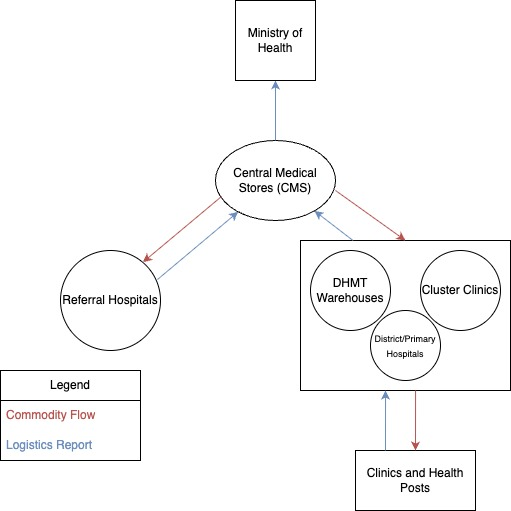
\includegraphics[width=0.6\textwidth]{figures/logistics_diagram}
    \caption{Simplified structure of Botswana's public pharmaceutical distribution system, adapted from the national logistics management manual and USAID GHSC-PSM \citep{ghsc2021botswana,botswanaSOP2019}. CMS procures centrally and distributes downstream through district warehouses to facilities.}
    \label{fig:logistics}
\end{figure}

To confirm the routing is realistic, we convert OSRM travel times to implied speeds; the distribution has a median near 58~km/h, with within-district trips mostly between 40 and 70~km/h and greater variability on longer inter-district routes over unpaved segments (Figure~\ref{fig:network}, right).

\begin{figure}[htbp]
    \centering
    \begin{subfigure}[b]{0.48\textwidth}
        \centering
\includegraphics[width=\textwidth]{figures/facility_type_counts}
        \caption{Facility counts by type.}
    \end{subfigure}\hfill
    \begin{subfigure}[b]{0.48\textwidth}
        \centering
\includegraphics[width=\textwidth]{figures/speed_distribution}
        \caption{Implied speeds from OSRM routes.}
    \end{subfigure}
    \caption{Network composition and routing validation. Left: the 614 nodes by service-delivery type. Right: implied speeds (distance divided by travel time) across all origin--destination pairs, confirming realistic travel dynamics on Botswana's mixed road network.}
    \label{fig:network}
\end{figure}

\subsection{Notation}
\label{sec:notation}

The problem data are as follows.
For each arc $(i,j) \in A$, the parameter $\text{Dist}_{ij}$ is the road distance and $v$ the per-unit transport cost.
For each node $n$ and class $k$, the parameter $\Delta_{n,k}$ is the penalty per unit of unmet demand and $h$ the per-unit holding cost carried to the next period.
Each facility has storage capacity $s_n$, each vehicle trip has shipment capacity $\text{cap}$, and $M$ is a large constant used in activation constraints.
The realized demand for class $k$ at node $n$ in period $t$ is $D_{n,k}^{(t)}$.

The decision variables, chosen at the start of each period, are the shipment $F_{(i,j),k}^{(t)}$ of class $k$ on arc $(i,j)$; the number of vehicle trips $\lambda_{(i,j)}^{(t)} \in \integers_+$ on that arc and a binary activation $y_{(i,j)}^{(t)}$; the procurement quantity $q_k^{(t)}$ at CMS; and, resolved at the end of the period, the ending inventory $I_{n,k}^{(t+1)}$ and unmet demand $U_{n,k}^{(t)}$.
We write $\bar D_{n,k}^{(t)}$ for the nominal (forecast) demand; the robust extension of \Sec\ref{sec:robust} introduces the deviation $\xi_{n,k}^{(t)}$, its bound $\sigma_{n,k}^{(t)}$, and the budget $\Gamma$.

\subsection{Deterministic Baseline}
\label{sec:baseline}

The deterministic model treats demand as known and equal to its nominal value, $D_{n,k}^{(t)} = \bar D_{n,k}^{(t)}$.
It minimizes total transport, shortage, holding, and procurement cost,
\begin{equation}
\min \;
v \sum_{(i,j)\in A} \text{Dist}_{ij}\,\lambda_{(i,j)}^{(t)}
+ \sum_{n\in N}\sum_{k} \left( \Delta_{n,k} U_{n,k}^{(t)} + h\, I^{(t+1)}_{n,k}\right)
+ \sum_{k} c_k^{\text{proc}}\, q_k^{(t)},
\label{eq:baseline_obj}
\end{equation}
subject to inventory balance at every non-CMS node and at CMS,
\begin{align}
I^{(t+1)}_{n,k} &= I^{(t)}_{n,k}
+ \textstyle\sum_{j:(j,n)\in A} F_{(j,n),k}^{(t)}
- \sum_{m:(n,m)\in A} F_{(n,m),k}^{(t)}
- D_{n,k}^{(t)} + U_{n,k}^{(t)},
&& n \neq 0, \label{eq:balance}\\
I^{(t+1)}_{0,k} &= I^{(t)}_{0,k} + q_k^{(t)}
- \textstyle\sum_{m:(0,m)\in A} F_{(0,m),k}^{(t)},
\label{eq:balance_cms}
\end{align}
a shipment-availability constraint ensuring outflow never exceeds stock on hand plus inflow and procurement,
\begin{equation}
\textstyle\sum_{m:(n,m)\in A} F_{(n,m),k}^{(t)}
\;\le\;
I_{n,k}^{(t)} + \sum_{j:(j,n)\in A} F_{(j,n),k}^{(t)}
+ \mathbf{1}_{\{n=0\}}\, q_k^{(t)},
\label{eq:availability}
\end{equation}
and arc-capacity, activation, and storage constraints,
\begin{equation}
\textstyle\sum_{k} F_{(i,j),k}^{(t)} \le \text{cap}\,\lambda_{(i,j)}^{(t)}, \quad
\lambda_{(i,j)}^{(t)} \le M\, y_{(i,j)}^{(t)}, \quad
\textstyle\sum_{k} I^{(t+1)}_{n,k} \le s_n,
\label{eq:capacity}
\end{equation}
together with nonnegativity of $F, I, U, q$, integrality of $\lambda$, and $y \in \{0,1\}$, for all applicable $n, k, (i,j)$.
Each period follows a fixed information timeline.
At the start of period $t$ the agency observes the inventory $I_{n,k}^{(t)}$ and commits the procurement $q_k^{(t)}$ and the routing decisions $\lambda_{(i,j)}^{(t)}$ and $y_{(i,j)}^{(t)}$.
Facilities then submit requisitions, which reveal the demand deviation for the period before vehicles are dispatched.
Shipments leave against those requisitions, demand is served, and unmet demand and ending inventory are determined at the close of the period.
The deterministic policy ignores the requisition signal and plans on nominal demand throughout; the adjustable policy of \Sec\ref{sec:adr} uses it, and we return to that distinction in \Sec\ref{sec:adr}.
This deterministic program is the benchmark against which we measure the value of hedging.

% ============================ ROBUST FORMULATION ============================
\section{Robust and Adjustable Robust Formulations}
\label{sec:robust}

The deterministic model presumes demand is known.
In practice it is not, and the central methodological question of the paper is how the agency should hedge.
This section develops that hedge in three steps: a budgeted uncertainty set, a static robust counterpart, and an affinely-adjustable policy whose tractable reformulation is the paper's technical core.

\subsection{Budgeted Uncertainty Set}
\label{sec:uncertainty}

We write demand as a nominal value plus a bounded deviation, $D_{n,k}^{(t)} = \bar D_{n,k}^{(t)} + \xi_{n,k}^{(t)}$, and require feasibility for every deviation in the budgeted set
\begin{equation}
\mathcal{U}^{(k)} = \left\{ \xi : \; |\xi_{n,k}^{(t)}| \le \sigma_{n,k}^{(t)} \;\; \forall n, \quad
\textstyle\sum_{n\in N} |\xi_{n,k}^{(t)}| / \sigma_{n,k}^{(t)} \le \Gamma \right\}.
\label{eq:uncertaintyset}
\end{equation}
The bound $\sigma_{n,k}^{(t)}$ is the largest plausible deviation at node $n$, calibrated in \Sec\ref{sec:demand} from the demand model's variance.
The budget $\Gamma$ caps how many nodes may simultaneously realize a worst-case deviation, and is the single knob trading conservatism against cost \citep{bertsim04}: $\Gamma = 0$ recovers the deterministic model, while large $\Gamma$ hedges against all nodes deviating at once.
The budget also carries a probabilistic reading.
For a constraint with $n$ uncertain coefficients, \citet{bertsim04} bound the probability of violation by $\exp(-\Gamma^{2}/2n)$.
With the $43$ nodes of the Gaborone instance, the setting $\Gamma = 10$ used below corresponds to a bound of roughly $31\%$, and $\Gamma \approx 16$ would be required for $5\%$.
Section~EC.4 reports performance across $\Gamma \in [1, 50]$, which spans this range.
Demand drawn from the negative-binomial model of \Sec\ref{sec:demand} is unbounded and so falls outside $\mathcal{U}^{(k)}$ in most periods.
The improvements we report should therefore be read as the effect of the protective stock positioning that the robust formulation induces, rather than as a coverage guarantee.

\subsection{Static Robust Counterpart}
\label{sec:static}

The static robust policy fixes all shipments before any demand is observed and requires every constraint that contains $\xi$ to hold for all $\xi \in \mathcal{U}^{(k)}$.
Because $\xi$ enters the inventory balance \eqref{eq:balance} and the availability constraint \eqref{eq:availability} linearly, each robust constraint is a semi-infinite linear inequality whose worst case is attained on $\mathcal{U}^{(k)}$.
Standard duality of the budgeted set \citep{bertsim04,bental} replaces each such constraint by a finite system of linear inequalities in auxiliary dual variables, giving a mixed-integer program of the same class as the deterministic model.
We use this static robust policy as an intermediate benchmark; the derivation parallels the adjustable case below and is given in the e-companion.

\subsection{Affine Decision Rules}
\label{sec:adr}

The static policy is conservative because it cannot use information that arrives during the horizon.
We relax it by letting each shipment respond affinely to the realized deviation.
At the start of each period the agency commits to a nominal shipment $\bar F_{(u,v),k}^{(t)}$ and a recourse coefficient $\alpha_{(u,v),k}^{(t)}$, and the executed shipment is
\begin{equation}
F_{(u,v),k}^{(t)}(\xi) = \bar F_{(u,v),k}^{(t)} + \alpha_{(u,v),k}^{(t)}\, \xi_{v,k}^{(t)}.
\label{eq:adr}
\end{equation}
Both $\bar F$ and $\alpha$ are chosen before any requisition arrives, and the executed shipment uses only the current period's requisition, so the policy never anticipates future periods.
It is the best \emph{linear} response to the signal as a function of the uncertainty set, and it reduces to the static policy when $\alpha = 0$.
The rule is deliberately restricted: a shipment responds only to the deviation at its own destination, in its own class, in the current period, rather than to the full history of observations.
This keeps the reformulation of \Sec\ref{sec:reformulation} linear in the network size, at the cost of some adaptivity.
Because a negative shipment has no physical meaning, we implement the truncation $F_{(u,v),k}^{(t)}(\xi) = \big(\bar F_{(u,v),k}^{(t)} + \alpha_{(u,v),k}^{(t)}\xi_{v,k}^{(t)}\big)^{+}$.
The truncation is inactive in practice: it binds on $0.03\%$ of arc--class--periods and affects $0.004\%$ of shipped volume in the Gaborone instance.
Substituting \eqref{eq:adr} into the inventory balance, availability, and capacity constraints and collecting the terms in $\xi$ turns each into a robust inequality of the form ``worst-case linear function of $\xi$ over $\mathcal{U}^{(k)}$ $\le$ slack,'' which is the object we dualize.

\subsection{Tractable Single-Level Reformulation}
\label{sec:reformulation}

The affinely-adjustable problem, written directly, is a min--max with an inner maximization over $\mathcal{U}^{(k)}$ inside every robust constraint.
Our main methodological result eliminates that inner problem.

\begin{proposition}[Tractable reformulation]
\label{prop:reformulation}
For the budgeted uncertainty set \eqref{eq:uncertaintyset} and the affine decision rule \eqref{eq:adr}, each robust constraint of the adjustable problem is equivalent to a finite set of linear inequalities in the original variables and a collection of nonnegative dual variables (one budget multiplier and two deviation multipliers per node--class, and their analogues for the availability and capacity constraints).
The adjustable robust allocation problem therefore admits an exact single-level mixed-integer linear reformulation whose size grows linearly in $|N|$, $|A|$, and $K$.
\end{proposition}

The proof dualizes the inner maximization using the Bertsimas--Sim representation of $\mathcal{U}^{(k)}$ and linear programming duality; we carry it out in full in Section~EC.1 of the e-companion, where the complete constraint system is stated.
Proposition~\ref{prop:reformulation} is what makes the framework usable: a naive formulation that retains the min--max structure is intractable at national scale, whereas the reformulated program is an ordinary mixed-integer program.
We solve it with off-the-shelf solvers \citep{gurobi,mosek}.

To reach national scale we add one further step.
Rather than solve a single program over all 614 facilities, we decompose by district and solve 18 independent subproblems.
This is partly computational, since each subproblem is far smaller, and partly a choice about how service is distributed across districts.
At national scale we also relax the vehicle-dispatch integrality to keep the subproblems tractable.
The next subsection makes the distributional choice explicit.

\subsection{The Equity Criterion}
\label{sec:equity}

A cost-minimizing allocation treats a unit of unmet demand as equally costly wherever it occurs, so it is indifferent between spreading shortfalls evenly and concentrating them in a few districts.
Whether that indifference is acceptable is a distributional question, and answering it requires stating what we mean by an equitable allocation.
We do so here in the language of \citet{bft11} and \citet{bft12}.

Let $\mathcal{D}$ index the districts, and let
\begin{equation}
s_d \;=\; 1 \;-\;
\frac{\sum_{n \in d}\sum_{k,t} U_{n,k}^{(t)}}
     {\sum_{n \in d}\sum_{k,t} D_{n,k}^{(t)}}
\label{eq:service}
\end{equation}
denote the service level of district $d$, the fraction of its demand met over the horizon.
An allocation induces the service vector $s = (s_d)_{d \in \mathcal{D}}$, and an equity criterion is a rule for aggregating that vector into a single objective.
We adopt the $\alpha$-fairness family,
\begin{equation}
W_\alpha(s) \;=\;
\begin{cases}
\displaystyle\sum_{d \in \mathcal{D}} \frac{s_d^{\,1-\alpha}}{1-\alpha}, & \alpha \neq 1,\\[2ex]
\displaystyle\sum_{d \in \mathcal{D}} \log s_d, & \alpha = 1,
\end{cases}
\label{eq:alphafair}
\end{equation}
which spans the criteria of interest with one parameter: $\alpha = 0$ is utilitarian and maximizes total service, $\alpha = 1$ is proportional fairness, and $\alpha \to \infty$ is max-min fairness, which maximizes the service level of the worst-served district.
The cost of insisting on fairness is the price of fairness,
\begin{equation}
\mathrm{POF}(\alpha) \;=\;
\frac{\ones^{T} s^{\star}_{0} - \ones^{T} s^{\star}_{\alpha}}{\ones^{T} s^{\star}_{0}},
\label{eq:pof}
\end{equation}
the relative loss in total service from optimizing $W_\alpha$ rather than $W_0$ \citep{bft11}.

Two things follow, and we are careful to separate them.
First, the district decomposition is a \emph{procedural} equity mechanism rather than a solution to \eqref{eq:alphafair} for any $\alpha$.
Because the subproblems are independent, no shipment may cross a district boundary, so by construction the decomposition rules out allocations that raise total service by moving supply from one district to another, whatever their relative demand density.
It guarantees each district a dedicated allocation and dedicated transport, independent of its size.
Second, this guarantee is not the same as optimizing an outcome criterion, and it comes at an efficiency cost that we do not measure: we do not solve the pooled national program, so we do not report $\mathrm{POF}$ for our instances.
\Sec\ref{sec:cms-results} reports the service vector the decomposition induces, and \Sec\ref{sec:discussion} returns to what remains open.
\mynote{Solving the pooled instance and sweeping $\alpha$ over \eqref{eq:alphafair} would let us plot the efficiency-fairness frontier and place the decomposition on it. Deferred.}

% ============================ DEMAND MODEL ============================
\section{The Medical Demand Estimator}
\label{sec:demand}

The robust model requires two demand inputs: a nominal forecast $\bar D_{n,k}^{(t)}$ and a deviation bound $\sigma_{n,k}^{(t)}$.
Botswana, like many low- and middle-income settings, lacks facility-level, high-frequency prescribing records; the available evidence is demographic tabulations and periodic point-prevalence surveys (PPS) reporting aggregate infection and prescription counts.
We therefore estimate demand with a negative-binomial regression calibrated to these sources, the Medical Demand Estimator (MDE), and derive $\sigma$ from its fitted variance.
We state the estimator and its properties here and defer proofs to Section~EC.2 of the e-companion.

For region $r$ and age group $a$, let $N_{r,a}$ be the number of admissions, $\mu_{r,a}$ the incidence rate of infections requiring treatment, and $\delta_a$ the guideline dose (one shipment unit).
The true regional demand is $D_r^{\star} = \sum_a N_{r,a}\,\mu_{r,a}\,\delta_a$.
We observe survey counts $Y_{r,a,1},\dots,Y_{r,a,n}$, taken as independent draws from a negative-binomial law with mean $\mu_{r,a}$ and dispersion $\kappa>0$, and model the mean log-linearly, $\mu_{r,a} = \exp(x_{r,a}^{T}\beta)$, where $x_{r,a}$ collects region, age, facility-type, and infection-category indicators.
The counts $Y_{r,a,1},\dots,Y_{r,a,n}$ are the $n$ patients sampled within a single cross-sectional PPS, not repeated surveys over time, so the large-sample regime below is in the number of sampled patients.

The estimator plugs the negative-binomial maximum-likelihood fit $\hat\beta_n$ into the demand map: $\hat D_r = \sum_a N_{r,a}\,\delta_a\,\exp(x_{r,a}^{T}\hat\beta_n)$.
Two properties make it usable as a nominal forecast.

\begin{proposition}[Consistency]
\label{prop:consistency}
Under the negative-binomial generalized-linear-model assumptions and standard regularity conditions, $\hat D_r \to D_r^{\star}$ in probability as $n\to\infty$.
\end{proposition}

\begin{proposition}[Dependence-preserving aggregation]
\label{prop:aggregation}
Let $Y_{j,i}$ indicate that patient $j$ needs antimicrobial class $i$, with patient vectors independent across $j$ but arbitrarily dependent across classes within a patient.
Then the aggregate demand $D_i = \sum_{j=1}^{N} Y_{j,i}$ satisfies $\mathbb{E}[D_i] = N\,\mathbb{E}[Y_{1,i}]$ while permitting any covariance structure across classes.
\end{proposition}

Proposition~\ref{prop:consistency} justifies using the fitted map as a forecast; Proposition~\ref{prop:aggregation} justifies building demand from PPS-calibrated per-patient indicators without observing the joint distribution across drug classes, which the surveys do not report.
Because facility-level admissions are unobserved, we approximate them by apportioning district inpatient totals to facilities in proportion to catchment population, and scale to the planning horizon.

Finally, the negative-binomial variance sets the uncertainty bound.
Under the NB2 parameterization, $\mathrm{Var}(Y) = \mu + \mu^2/\kappa$, so we take
\begin{equation}
\sigma_{n,k}^{(t)} = \sqrt{\bar D_{n,k}^{(t)} + \big(\bar D_{n,k}^{(t)}\big)^2 / \kappa},
\label{eq:sigma}
\end{equation}
the standard deviation of demand, as the radius of the uncertainty set \eqref{eq:uncertaintyset}.
The single fitted PPS yields a large $\hat\kappa$ (near-Poisson variability); because this rests on one survey, we treat $\kappa$ as uncertain and report sensitivity across a range of values in \Sec\ref{sec:results}.

% ============================ NUMERICAL STUDY ============================
\section{Numerical Study}
\label{sec:results}

We evaluate three policies: the \emph{deterministic} baseline of \Sec\ref{sec:baseline}, which plans on nominal demand; the \emph{static robust} policy of \Sec\ref{sec:static}; and the adjustable \emph{ARO-ADR} policy of \Sec\ref{sec:adr}.
In each period the simulator draws demand, computes shipments under the policy, and rolls inventory forward by the balance equations; deviation bounds follow \eqref{eq:sigma}.
Demand is drawn from the fitted negative-binomial model, and all policies see identical realizations for comparability.
We report a Gaborone proof-of-concept, a national simulation, results driven by real procurement data, sensitivity analyses, and an epidemic-driven extension.

\subsection{Gaborone Proof-of-Concept}
\label{sec:gaborone}

We first study penicillin distribution across the Gaborone district, comprising CMS, Princess Marina Hospital, and downstream clinics and health posts, with $\Gamma = 10$ and $\kappa = 10$.
Each policy is evaluated over $R = 12$ independent demand realizations of $T = 100$ periods each, drawn from the fitted negative-binomial model and shared across policies so the comparison is paired.
Averages are taken within a realization and standard errors across them.
Taking standard errors across the periods of a single path would understate uncertainty, since inventory carried between periods makes them dependent.
Cost parameters are illustrative ($h=0.1$, $\Delta=100$, $c=1$ per unit).
The three policies diverge sharply.
The deterministic policy leaves on average about 13\% of demand unmet, with period-to-period shortfalls frequently above 20\%.
Static robust cuts this to roughly 3.6\% by pre-positioning stock against worst-case deviations, and ARO-ADR to roughly 2.0\% (Figure~\ref{fig:gaborone}).
\mynote{These three figures are the single-path values. Re-verify against the mean over the 12 replications once that run completes; the single path is replication 0, so any change should be small.}
The adaptive gain is cheap: relative to static robust, ARO-ADR removes about 42\% of the remaining unmet demand for a procurement increase of only about 1.5\%, because affine recourse lets shipments respond to realized demand rather than committing in advance.
Figure~\ref{fig:gabcost} makes the economics explicit.
The cost breakdown shows transport cost broadly similar across policies, so the performance gap is driven by inventory and shortage decisions rather than routing; the per-period net benefit of ARO-ADR over static robust (unmet demand eliminated minus added procurement) is positive in most periods; and the total objective under ARO-ADR is lowest, about 33\% below static robust and over 75\% below deterministic, since the shortage penalty dominates the objective.

\begin{figure}[htbp]
    \centering
    
\includegraphics[width=0.72\textwidth]{figures/unmetdemandaverage100gabs}
    \caption{Gaborone proof-of-concept: average unmet antimicrobial demand under the three policies. Each bar is the mean over $R = 12$ independent demand realizations of $T = 100$ periods, and the error bar is one standard error across those realizations. Adaptive recourse (ARO-ADR) achieves the lowest unmet demand.}
    \label{fig:gaborone}
\end{figure}

\begin{figure}[htbp]
    \centering
    \begin{subfigure}[b]{0.48\textwidth}
        \centering
\includegraphics[width=\textwidth]{figures/costbreakdown}
        \caption{Cost breakdown by component.}
    \end{subfigure}\hfill
    \begin{subfigure}[b]{0.48\textwidth}
        \centering
\includegraphics[width=\textwidth]{figures/costbenefit}
        \caption{Net benefit of ARO-ADR over static robust.}
    \end{subfigure}
    \vspace{0.5em}
    \begin{subfigure}[b]{0.6\textwidth}
        \centering
\includegraphics[width=\textwidth]{figures/objectivecomparison}
        \caption{Average total objective.}
    \end{subfigure}
    \caption{Economics of adaptive recourse in the Gaborone proof-of-concept. Transport cost is similar across policies (a), the per-period net benefit of ARO-ADR over static robust is positive in most periods (b), and ARO-ADR attains the lowest total objective (c).}
    \label{fig:gabcost}
\end{figure}

\subsection{National Simulation}
\label{sec:national}

We next solve the model for all 18 districts under the district decomposition of \Sec\ref{sec:reformulation}.
Table~\ref{tab:national} reports average per-period performance.
The ordering of the proof-of-concept persists at national scale: ARO-ADR reduces unmet demand to 1.9\%, an 86\% reduction relative to deterministic and 48\% relative to static robust, at a 0.9\% procurement premium over static robust under these illustrative unit costs, and a total objective 26\% below static robust.
Beyond the average, the geographic distribution matters: under ARO-ADR the worst-served district sits close to the national mean, whereas the deterministic policy concentrates shortfalls in high-demand districts (Figure~\ref{fig:heatmap}).
We quantify this in \Sec\ref{sec:cms-results}, where the effect is a uniform improvement in level rather than a reduction in relative inequality.

\begin{table}[t]
\centering
\caption{National simulation: average per-period performance across all 18 districts (illustrative unit costs).}
\label{tab:national}
\begin{tabular}{lccc}
\toprule
Policy & Avg.\ unmet demand (\%) & Avg.\ procurement cost & Avg.\ objective \\
\midrule
Deterministic  & 13.48 & 21{,}266 & 318{,}473 \\
Static robust  & 3.61  & 23{,}744 & 101{,}689 \\
ARO-ADR        & 1.88  & 23{,}967 & 75{,}072  \\
\bottomrule
\end{tabular}
\end{table}

\begin{figure}[htbp]
    \centering
    
\includegraphics[width=0.9\textwidth]{figures/botswana_heatmap}
    \caption{Average unmet demand by district under the three policies ($T=20$). ARO-ADR (right) is low everywhere, including in the worst-served districts; the deterministic policy (left) concentrates shortfalls. District names are omitted; the geography is identical in every panel.}
    \label{fig:heatmap}
\end{figure}

\subsection{Results on Real Procurement Data}
\label{sec:cms-results}

To test the policies on empirically grounded costs rather than illustrative ones, we drive the model with CMS's actual records for 84 antimicrobial products: average monthly consumption for the 2025--26 and 2026--27 planning horizons, and unit prices from CMS pricing records.
We simulate all 18 districts.
Table~\ref{tab:cms} reports the results.
The policy ordering is unchanged, and the coverage gains are if anything larger: ARO-ADR cuts unmet demand from 21.7\% (deterministic) to 3.4\% in 2025--26 and from 19.2\% to 2.8\% in 2026--27.
The procurement premium of ARO-ADR over static robust is now 6.5\% and 6.4\%, materially larger than the 0.9\% under illustrative costs, because the premium is a cost ratio and CMS's actual prices differ from the convenience value $c=1$.
We report both figures rather than the smaller illustrative one; the total objective remains lowest under ARO-ADR in both horizons, so the added procurement is more than repaid by avoided shortages.
The geographic pattern (Figure~\ref{fig:cmsmap}) mirrors the simulation.
In 2025--26 the deterministic policy leaves North East, Ghanzi, and Kgalagadi South at $29.6\%$, $27.2\%$, and $26.7\%$ unmet demand, while both robust policies, and ARO-ADR most of all, bring every district to a low level.
Two things the map can be read as showing are worth separating.
The improvement in level is large and reaches everywhere: the worst-served district improves from $29.6\%$ under the deterministic policy to $4.6\%$ under ARO-ADR, so no district is traded off against another.
In the language of \Sec\ref{sec:equity}, the max-min service level $\min_d s_d$ rises from $0.704$ to $0.954$, so the criterion at $\alpha \to \infty$ improves substantially.
Relative dispersion across districts, however, is largely unchanged.
The coefficient of variation of district unmet demand is $0.16$ under ARO-ADR against $0.18$ under deterministic, and the Gini coefficient is $0.08$ against $0.10$.
We therefore claim a uniform improvement in service level, not a reduction in relative inequality.
A disaggregated breakdown by cost component and district is given in Section~EC.4.

\begin{table}[t]
\centering
\caption{Real CMS procurement data: average unmet demand (\%), procurement cost (BWP), and objective by model and scenario across all 18 districts.}
\label{tab:cms}
\begin{tabular}{llrrr}
\toprule
Scenario & Model & Avg.\ unmet (\%) & Avg.\ procurement & Avg.\ objective \\
\midrule
2025--26 & Deterministic & 21.72 & 143{,}445.95 & 407{,}746.36 \\
         & Static robust & 7.05  & 182{,}194.06 & 274{,}824.08 \\
         & ARO-ADR       & 3.40  & 194{,}026.78 & 216{,}719.85 \\
\midrule
2026--27 & Deterministic & 19.17 & 208{,}293.50 & 532{,}339.06 \\
         & Static robust & 5.98  & 252{,}237.42 & 361{,}051.61 \\
         & ARO-ADR       & 2.76  & 268{,}293.00 & 294{,}511.09 \\
\bottomrule
\end{tabular}
\end{table}

\begin{figure}[htbp]
    \centering
    
\includegraphics[width=0.62\textwidth]{figures/cms_unmet_map}
    \caption{Real CMS procurement data: average unmet antimicrobial demand (\%) by district. Rows are policies (deterministic, static robust, ARO-ADR); columns are the 2025--26 and 2026--27 scenarios. ARO-ADR achieves low unmet demand in every district. District names are omitted; the geography is identical in every panel.}
    \label{fig:cmsmap}
\end{figure}

\subsection{Sensitivity: When Is Adaptivity Worth It?}
\label{sec:sensitivity}

Two parameters govern the robust policies: the dispersion $\kappa$, which sets the uncertainty radius through \eqref{eq:sigma}, and the budget $\Gamma$.
Because $\kappa$ is estimated from a single survey, we vary the true and assumed $\kappa$ over a grid (Figure~\ref{fig:kappa}).
On the diagonal (correct $\kappa$) the ordering holds at every volatility level.
Off the diagonal, misspecification hurts static robust sharply, over-assuming $\kappa$ shrinks the uncertainty set and both robust policies under-hedge, while ARO-ADR degrades gracefully because its recourse adapts to realized deviations even when the nominal set is miscalibrated.
Adaptivity is thus not only a performance improvement but a hedge against getting $\kappa$ wrong.

\begin{figure}[htbp]
    \centering
    
\includegraphics[width=0.85\textwidth]{figures/kappa}
    \caption{Sensitivity to the dispersion parameter. Rows: true $\kappa$ generating demand; columns: assumed $\kappa$ calibrating the uncertainty set. ARO-ADR degrades most gracefully under misspecification.}
    \label{fig:kappa}
\end{figure}

Varying $\Gamma$ (Section~EC.4) shows the value of adaptivity concentrating in an identifiable regime: the ARO-ADR advantage over static robust is largest at small $\Gamma$ and high variability (low $\kappa$), and shrinks as $\Gamma$ grows, because a large budget forces the optimizer to worst-case over so many nodes that it suppresses the adaptive component and the policy collapses toward the static one.
The managerial reading is direct: invest in adaptive recourse when demand is volatile and the uncertainty budget is moderate; a simpler static policy suffices otherwise.

Finally, we vary the shortage penalty $\Delta$ over $[0.1, 100]$ at fixed unit procurement cost $1$ (Section~EC.4).
The response is governed by a threshold near the procurement cost.
When $\Delta$ is at or below unit cost, serving demand is not cost-effective and unmet demand rises sharply; once $\Delta$ rises well above it (here beyond roughly $10$), realized unmet demand saturates and becomes essentially invariant to the penalty, because achievable service is then pinned by physical capacity and, for the robust policies, the uncertainty set, none of which depend on $\Delta$.
Since the clinical cost of an antimicrobial stockout far exceeds unit procurement, the operationally relevant regime is exactly this saturated one, in which the policy ordering holds and the recommended policy is insensitive to the exact penalty an agency chooses.

\subsection{Extension: Epidemic-Driven Demand}
\label{sec:seir}

The evaluation so far treats demand as statistically uncertain but exogenous.
As an extension, we make demand epidemiologically driven by coupling the allocation model to a two-strain compartmental model at Princess Marina Hospital, calibrated to gram-negative bloodstream infection dynamics.
The two strains are drug-susceptible (DS), treated with first-line cephalosporins, and drug-resistant (DR), treated with second-line carbapenems.
Treatment intensity is tied to realized supply: the DS and DR treatment rates scale with the delivered fractions of cephalosporins and carbapenems, saturating at their nominal levels.
A stockout therefore suppresses treatment, prolonging infectiousness and feeding a resistance-amplification pathway in which imperfectly treated DS infections convert to DR.
The coupling runs closed-loop, one period at a time.
In each period we solve the allocation problem, observe how much cephalosporin and carbapenem actually reached the hospital, advance the compartmental system under that realized supply, and draw the next period's demand from the updated infectious population.
A policy therefore faces the demand its own stockouts create, which is what we mean by saying that distribution failures and disease dynamics co-evolve.
Note that the allocation models themselves do not anticipate this feedback: they optimize against the demand they are given, and the feedback enters through the environment rather than the objective.
We present this as a proof-of-concept coupling rather than a validated epidemiological model; the full compartmental system and its calibration are in Section~EC.3.

Over a two-year horizon the policy ordering is preserved: ARO-ADR holds average unmet demand near 0.1\%, against 3.5\% for static robust and 12.7\% for deterministic (Table~\ref{tab:epi}), with near-zero shortfalls even during epidemic demand spikes that push the deterministic policy above 25\%.
The effect on resistance is more subtle and we are careful not to overclaim it.
Better-supplied policies clear both strains faster, so they end with a lower \emph{absolute} resistant burden.
But they also show a marginally higher resistant \emph{fraction}, because faster clearance of susceptible infections shrinks the denominator; extending the compartmental model to a 50-year horizon (Section~EC.3) shows this fraction gap is a small, persistent denominator effect that never reverses into greater resistance emergence.
The framework's benefits are therefore best read as coverage gains, substantial and robust reductions in unmet demand, rather than as changes to long-run resistance dynamics.

\begin{table}[t]
\centering
\caption{Epidemic-driven demand at Princess Marina Hospital ($T=52$ biweekly periods): allocation-policy performance.}
\label{tab:epi}
\begin{tabular}{lrrr}
\toprule
Policy & Avg.\ unmet (\%) & Avg.\ objective & Avg.\ procurement \\
\midrule
Deterministic & 12.73 & 38{,}710 & 2{,}430 \\
Static robust &  3.54 & 13{,}595 & 2{,}722 \\
ARO-ADR       &  0.08 &  3{,}630 & 2{,}817 \\
\bottomrule
\end{tabular}
\end{table}

\begin{figure}[htbp]
    \centering
    
\includegraphics[width=\textwidth]{figures/epidemic_gaborone_results}
    \caption{Epidemic-driven demand at Princess Marina Hospital over a two-year horizon. \textbf{Left:} unmet antimicrobial demand over time. \textbf{Center:} SEIR compartment trajectories under ARO-ADR, with both infectious populations declining under adequate supply. \textbf{Right:} average unmet demand by policy. The extended resistance analysis is deferred to Section~EC.3.}
    \label{fig:epi}
\end{figure}

% ============================ DISCUSSION ============================
\section{Managerial Implications and Limitations}
\label{sec:discussion}

\paragraph{What an agency should take away.}
Three findings are directly actionable.
First, adaptive recourse is worth adopting: it cuts unmet demand by about three-quarters relative to the deterministic planning that characterizes current practice, at a procurement premium in the single digits, and the added procurement is repaid by avoided shortages in every scenario we study.
Second, the gains are broad rather than concentrated: solving per district lifts every district's service level, including the worst-served, so an agency does not trade rural coverage for urban.
The improvement is in the level of service everywhere, not in the relative dispersion across districts, and \Sec\ref{sec:equity} makes that distinction precise.
Third, calibration is forgiving in the ways that matter and demanding in the ways one can prepare for.
The recommended policy is insensitive to the shortage penalty in the operationally relevant regime, so an agency need not pin down the clinical cost of a stockout precisely; but performance does depend on the dispersion $\kappa$ and budget $\Gamma$, and the value of adaptivity is largest under high volatility and a moderate budget, which is exactly where we recommend investing in it.

\paragraph{Deployability.}
The framework is designed as decision support that an agency can drive with data it already holds or can assemble: a facility list with locations, a routing engine, catchment populations, and consumption records of the kind CMS provided.
The tractable reformulation and district decomposition keep solve times within a replenishment cycle, and the model accepts richer demand inputs without structural change as data improve.

\paragraph{Limitations.}
Several caveats bound the claims.
The demand estimator is calibrated to a single inpatient point-prevalence survey from one district, so the forecasts are best read as lower bounds on true facility need rather than complete demand; the optimization structure is unchanged by better inputs, but the numbers would move.
The results are simulation-based: we evaluate policies on real cost and consumption data, but no policy has been deployed, so we observe modeled rather than realized outcomes.
The epidemic coupling is a proof of concept with parameters partly borrowed from the literature, and its resistance results should be read as coverage effects, not validated resistance forecasts.
Finally, we take procurement prices and routing distances as fixed and known; supply-side uncertainty in lead times and prices, which we do not model, is a natural and important extension.
Equity enters our design procedurally, through the district decomposition, rather than as a criterion optimized over outcomes.
\Sec\ref{sec:equity} states the criterion we would optimize, the $\alpha$-fairness family of \citet{bft12}, and the efficiency loss we would report, the price of fairness of \citet{bft11}.
We do neither here: we do not solve the pooled national program, so the position of our allocation on the efficiency-fairness frontier is unknown, and characterizing it is the most immediate extension of this work.

% ============================ CONCLUSION ============================
\section{Conclusion}
\label{sec:conclusion}

We have developed a robust, adjustable multi-echelon model for allocating antimicrobials across a national distribution network under uncertain demand, and shown that its tractable single-level reformulation scales to a country-sized problem while a district decomposition gives every district a dedicated allocation.
We state the equity criterion this mechanism is and is not solving, and leave the position of our allocation on the efficiency-fairness frontier as the immediate next question.
On real procurement data from Botswana's Central Medical Stores, adaptive recourse delivers large reductions in unmet demand in every district, including the worst-served, for a modest procurement premium, and we characterized when adaptivity earns its cost and why the recommended policy is insensitive to the shortage penalty.
The problem we study, a central agency distributing essential medicines over a heterogeneous network under demand it cannot fully observe, is common across import-dependent health systems, and the framework transfers wherever comparable facility, routing, and consumption data can be assembled.
Its benefits are best understood as coverage gains: getting antimicrobials to the point of care more reliably, more evenly, and at acceptable cost.

% ============================ BIBLIOGRAPHY ============================
\bibliography{bibliography}

\end{document}
